\section{title}

\subsection{subsection}

a equation
$$
p(y=c|x, w) = softmax(f(x))
$$
. The $w$ is the parameters of a neural network, and $f$ is the output of the model. So for each input image, we can get a probability vector $p(y=c|x, w)$.

The authors evaluated the models on MNIST (\cite{mnist}), CIFAR-10 (\cite{cifar10}), a diabetic retinopathy dataset (\cite{retinopathy}) and ImageNet(\cite{resnet}). Shaded areas in the plots denote $\pm$ one standard deviation.


\begin{enumerate}
    \item MNIST: The network architecture for MNIST, referred to as “S-CNN”, contains two convolutional layers and one dense layer. It is the same as the Keras MNIST CNN implementation (\cite{keras_cnn}).
    \item CIFAR-10: The authors experiment a CNN model with four convolutional layers and one dense layer as the Keras CIFAR CNN implementation (\cite{keras_cnn}), which we refer to as “K-CNN”. 
    
    Additionally they also evaluate with DenseNet-121 (k = 12, with bottleneck), using the learning rate schedule as proposed in \cite{denseNet}. 
    \item diabetic retinopathy dataset: Details for the inceptionV3 architecture are described in section 4.5.
    \item ImageNet: ResNet-50\cite{resnet} is used in the experiments. The network is trained for 100 epochs without data augmentation using stochastic gradient descent. The initial learning rate of 0.1 is changed to 0.01 at epoch 50, and 0.001 at epoch 75. The initial 40,000 images are class-balanced.
\end{enumerate}

Figure.\ref{figure1} is show below:

\begin{figure}[ht!]
    \centering
    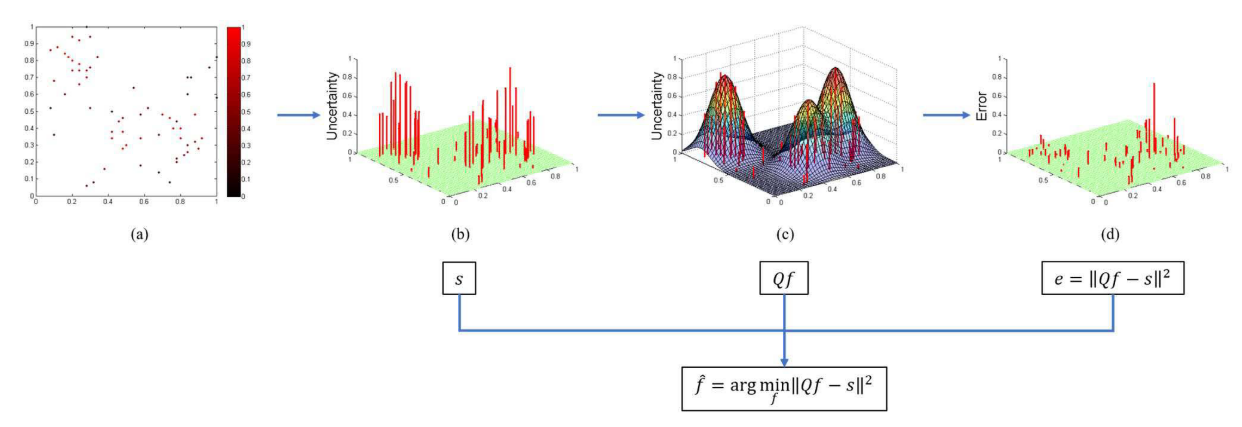
\includegraphics[width=15.4cm]{sparse_overview.png}
    \caption{overview}
    \label{figure1}
\end{figure}